\documentclass[a4paper, 10pt, twocolumn]{article}

\usepackage[utf8]{inputenc}
\usepackage[T1]{fontenc}

\usepackage[english]{babel}

\usepackage{graphicx}
\usepackage{amsmath}
\usepackage{amssymb}
\usepackage{amsthm}

\usepackage{txfonts}

\usepackage[left=1.3cm, 
						right=1.3cm, 
						top=3.0cm, 
						bottom=2.5cm,
						]{geometry}

\usepackage{url}
\usepackage{booktabs}
\usepackage{multirow}
\usepackage{array}
\usepackage{dcolumn}

\usepackage{titlesec}
\titleformat*{\subsubsection}{\itshape}

\usepackage[justification=centered]{caption}
\captionsetup[table]{singlelinecheck=off,justification=raggedright}
\captionsetup[figure]{singlelinecheck=off,justification=raggedright}

\addto\captionsslovak{
\def\tablename{Tab.}
\def\figurename{Obr.}
}

\hyphenpenalty=6000
\tolerance=6000

\usepackage{listings}
\usepackage{xcolor}

\definecolor{codegray}{rgb}{0.5,0.5,0.5}
\definecolor{codeblue}{rgb}{0,0,0.8}
\definecolor{codegreen}{rgb}{0,0.5,0}

\lstset{
    language=Python,
    basicstyle=\ttfamily\small,
    numbers=left,
    numberstyle=\tiny\color{codegray},
    keywordstyle=\color{codeblue},
    commentstyle=\color{codegreen},
    stringstyle=\color{codeblue},
    breaklines=true,
    frame=single,
    captionpos=b,
    tabsize=4,
    showstringspaces=false
}



\begin{document}

\pagestyle{empty}

\setlength\parindent{0.8cm}





\twocolumn[{%
\centering

\parbox{17cm}{%
\centering

\fontsize{20}{24}\selectfont%

\vspace{18pt}

Data science application in ICT}

\vspace{18pt}

\fontsize{12}{15}\selectfont%

Dmitrii Savin, 

\vspace{12pt}

\fontsize{10}{12}\selectfont%

$^1$Institute of Multimedia Information and Communication Technologies, FEI STU in Bratislava\\


\vspace{6pt}

xsavin@stuba.sk

\vspace{12pt}

\vspace{4mm} %finetune

}]




\noindent
\textbf{Abstract – This paper demonstrates the vital role of Data Science in ICT by solving complex problems through advanced analytics. Using the “5G Resource Allocation Dataset” \cite{SOBHY2023} we explore resource distribution in 5G networks. The study applies data cleaning, feature engineering, and machine learning to optimize allocation. The practical section includes Python implementations with pandas and the RandomForest \cite{RandomForestRegressor} algorithm to calculate resource shares, sort application types, and predict allocations based on network parameters.}


\section{Introduction}

Data Science has emerged as a pivotal field within Information and Communication Technologies (ICT), empowering professionals to extract insights and make data-driven decisions. With the increasing complexity of digital infrastructures and the explosive growth of data, Data Science offers robust methods to analyze, model, and optimize operations across diverse sectors.

The advent of 5G networks brings revolutionary improvements in connectivity, speed, and latency. However, dynamically allocating network resources in such environments remains a complex challenge. 

\subsection{Data Science Methodology}

At the heart of this work is a Data Science workflow that includes key steps: Data Collection and Cleaning, which involves handling raw datasets and ensuring that missing or inconsistent data are managed effectively; Feature Engineering, which focuses on extracting and transforming relevant features from the dataset such as signal strength, latency, and bandwidth requirements; and Statistical Analysis and Modeling, which utilizes statistical methods and machine learning algorithms (like RandomForest) to build predictive models.

\subsection{Present usage of 5G networks}
The analysis of the dataset reveals current trends in mobile network usage. The diversity of application types reflects the wide range of tasks that 5G networks must support.
\begin{itemize}
    \item \textbf{Video Communication and Multimedia:} Applications for video calls and streaming video require high bandwidth, minimal latency, and a reliable connection due to the real-time transmission of large volumes of data.
    \item \textbf{IoT Devices:} Applications related to the Internet of Things exhibit stable but less bandwidth-demanding resource allocation. Although these devices transmit relatively small amounts of data, they require continuous connectivity and energy efficiency.
    \item \textbf{Online Gaming and Social Networks:} These application categories have unique requirements — from low latency to high-speed data transmission — which necessitate dynamic allocation of network resources.
\end{itemize}

\subsection{Rapid Development of 5G Networks}

Since early trials in the 2010s and the establishment of standards by organizations like 3GPP, 5G quickly evolved into a global network by 2019, driving innovations with its unprecedented speeds and low latency that now power smart cities, IoT, and autonomous systems.









\section{Theoretical part and it’s components}

In the theoretical part of this study, fundamental concepts of dynamic resource allocation in ICT were employed, along with statistical analysis and machine learning methods. Core theoretical materials include a dataset with different key parameters such as signal strength, latency, and bandwidth requirements. 

These concepts guided the development of our analytical approach and informed the design of the Python code, which implements functions for calculating resource allocation percentages, sorting by application type, and training a RandomForest model for predictive analytics.


\subsection{Software used}
The study primarily relies on Python as the main software environment. We used the \textbf{Pandas} \cite{KaggleLearn} library that simplifies data manipulation and analysis. It introduces two primary data structures: the DataFrame, which organizes data in a tabular format with labeled axes, and the Series, a one-dimensional array with an associated index. These structures allow for intuitive data handling, enabling users to filter, merge, reshape, and aggregate data efficiently. Pandas also offers extensive support for reading from and writing to various file formats such as CSV, Excel, and SQL databases. Its seamless integration with libraries like NumPy and scikit-learn makes it an essential tool for building data-driven applications and performing exploratory data analysis.

\textbf{RandomForest}, a popular ensemble method available in scikit-learn, builds multiple decision trees during training and aggregates their predictions. For regression tasks, it computes the average of all tree outputs, while for classification tasks, it uses majority voting. This ensemble approach helps mitigate overfitting and improves prediction accuracy. In our work, we leverage the \textbf{RandomForestRegressor} to predict network resource allocation based on features like signal strength, latency, and bandwidth requirements, demonstrating the practical application of machine learning in optimizing ICT systems.

\section{Experimental approach and results}
\subsection{Key Analytical Functions}
Below is a list of essential functions used in the analysis, along with a brief description of their roles:

\begin{lstlisting}[caption={Random Forest Model Training}]
def train_random_forest_model(df, target_col='Resource Allocation', feature_cols=None, test_size=0.2, random_state=42):
    """
    Trains a RandomForestRegressor and prints the R² score.
    Returns the trained model and test data.
    """
    if feature_cols is None:
        feature_cols = df.select_dtypes(include=['float64', 'int64']).columns.drop(target_col).tolist()
    data = df.dropna(subset=[target_col] + feature_cols)
    X, y = data[feature_cols], data[target_col]
    X_train, X_test, y_train, y_test = train_test_split(X, y, test_size=test_size, random_state=random_state)
    model = RandomForestRegressor(random_state=random_state)
    model.fit(X_train, y_train)
    score = r2_score(y_test, model.predict(X_test))
    print(f"R² score: {score:.2f}")
    return model, (X_test, y_test), score
\end{lstlisting}


\newpage

\subsection{Results Visualization and Analysis}

\begin{figure}[h]
\centering

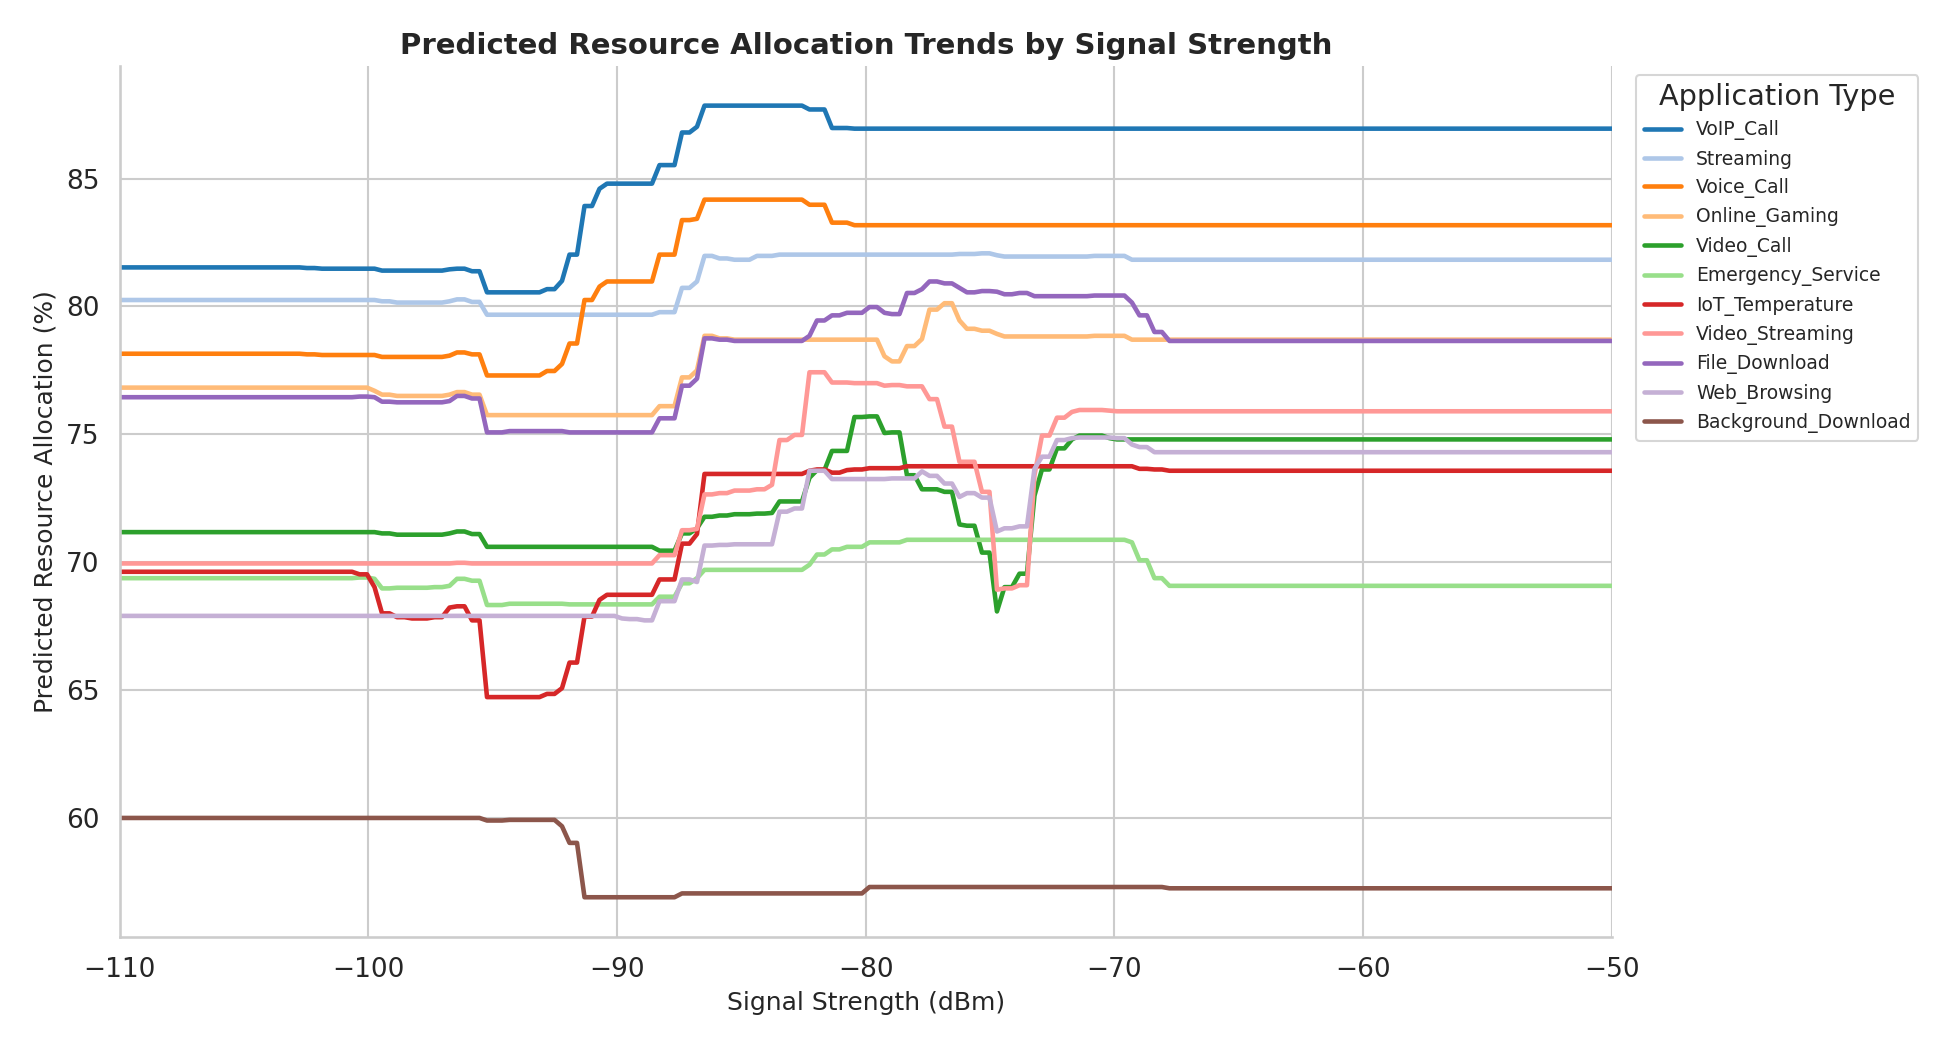
\includegraphics[width=\columnwidth]{fig1.png}

\caption{\centering Predicted resource allocation trends by signal strength.}
\label{figure1}

\end{figure}

As signal strength improves (from about –110 to –70 dBm), most applications receive more resources, with the largest increases for critical and interactive services (Video Call, Emergency Service, Online Gaming). Lower-priority apps (IoT, File Download) rise more gradually. 

The stepped changes indicate threshold splits from the RandomForest model. Overall, the model effectively reallocates resources, prioritizing high-demand applications as signal quality improves.

\begin{figure}[h]
\centering

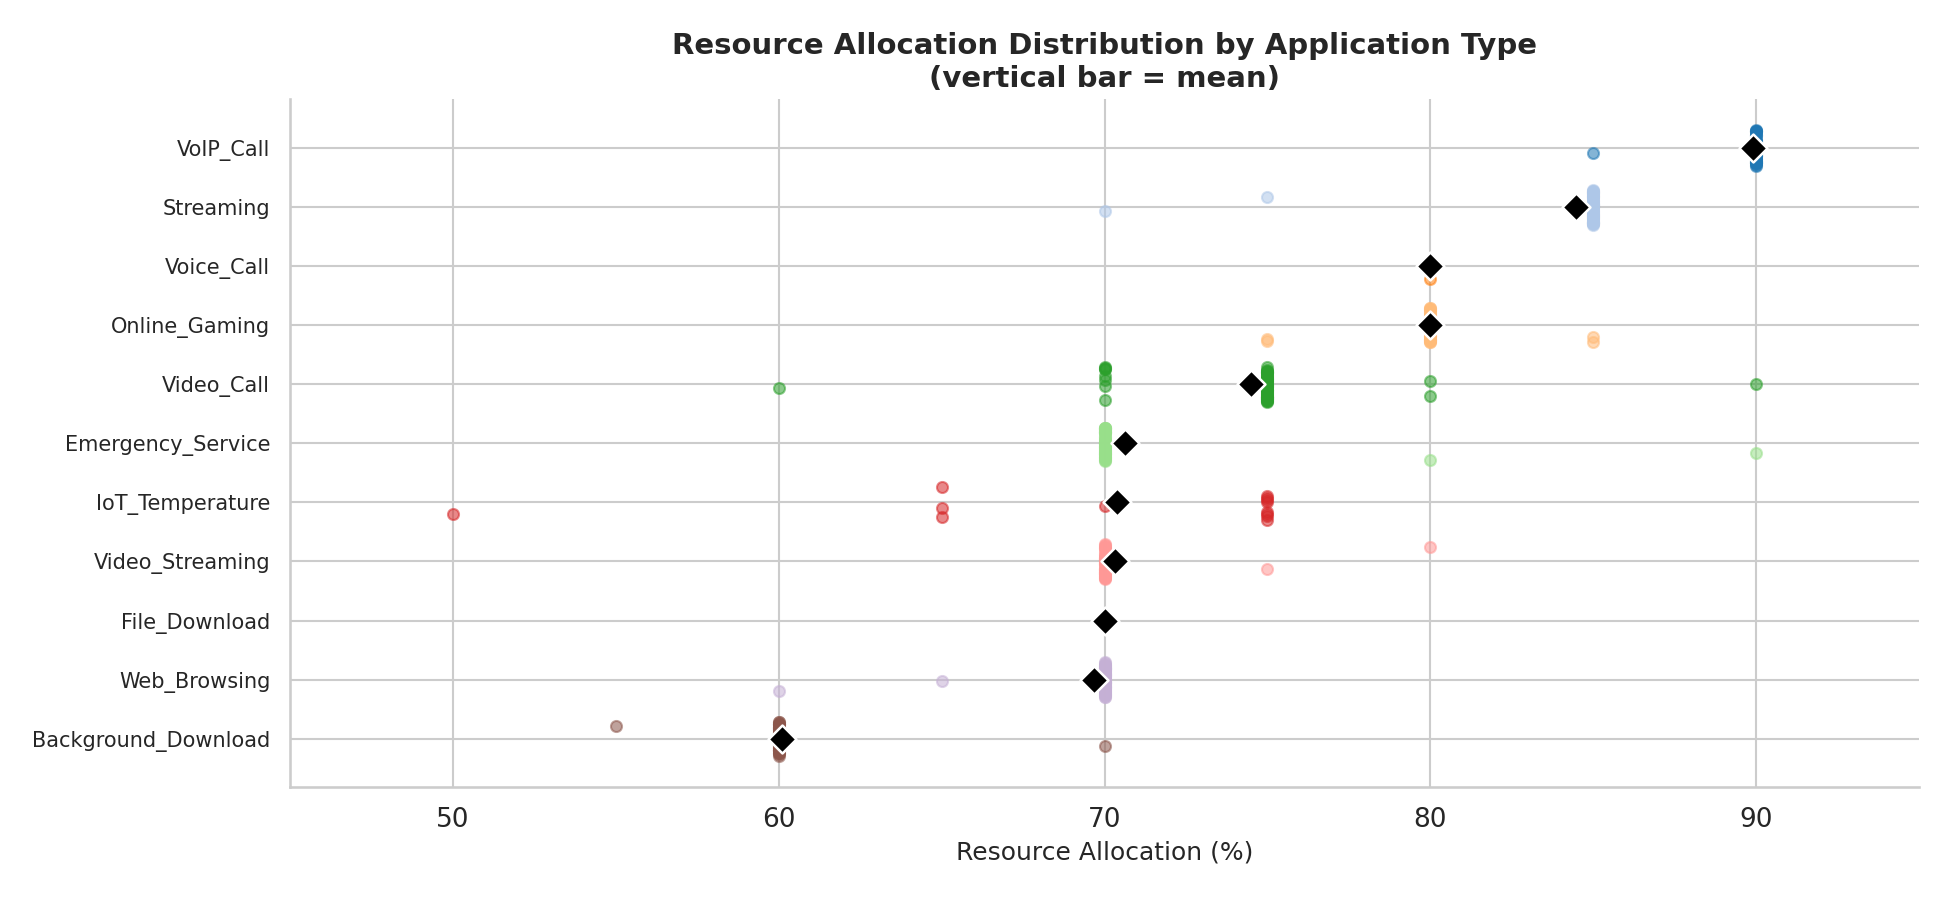
\includegraphics[width=\columnwidth]{fig2.png}

\caption{\centering Resource allocation distribution by application type.}
\label{figure2}

\end{figure}

This bar chart shows how resources are distributed across different application types. \textbf{VoIP Call}, \textbf{Video Call}, receive the highest allocations, suggesting a priority on real-time and critical services. Meanwhile, lower demands are allocated to IoT, file downloads, and certain streaming tasks, indicating that less urgent applications get fewer resources in this model.

\newpage

\begin{figure} [h]
    \centering
    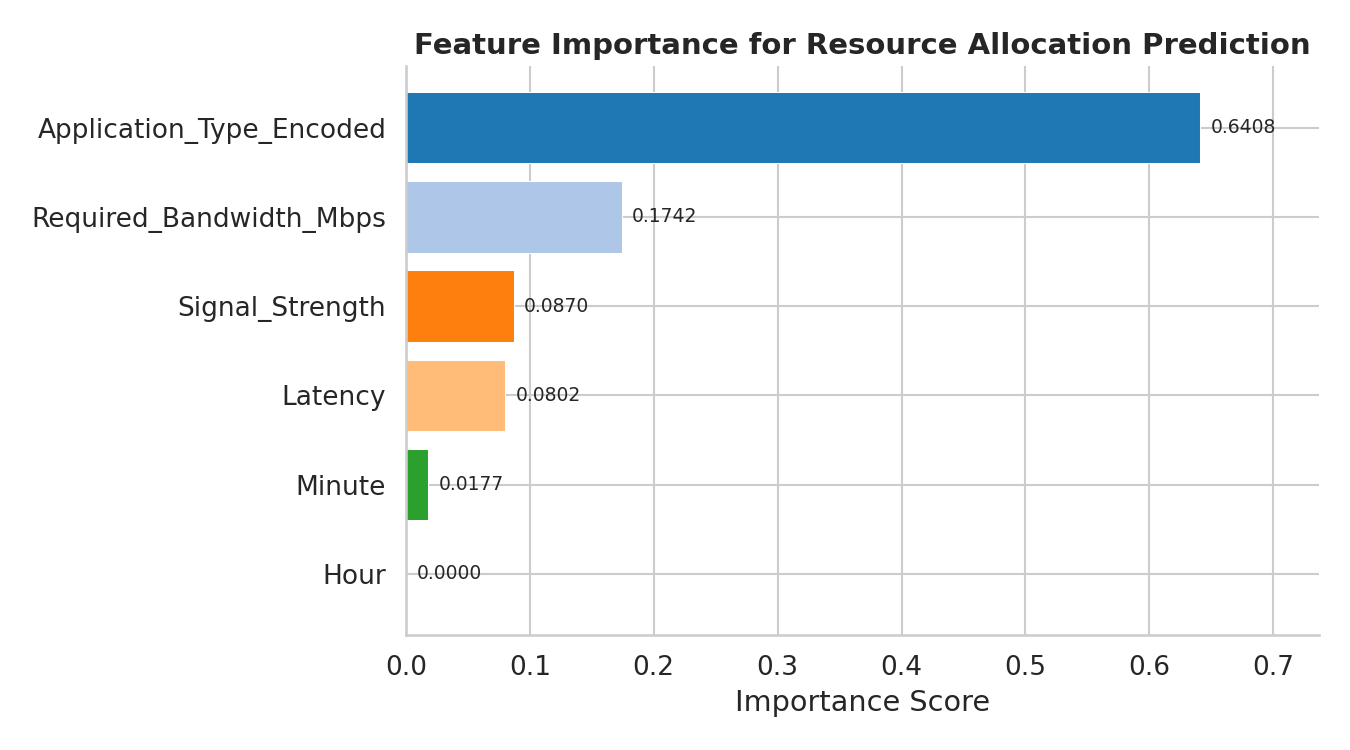
\includegraphics[width=\columnwidth]{fig3.png}
    \caption{\centering Feature Importance}
    \label{figure3}
\end{figure}

This bar chart highlights the importance of each feature in predicting resource allocation. The model relies most heavily on \textbf{Required Bandwidth} and \textbf{Application Type}, indicating that the nature of the application and its bandwidth needs drive the majority of allocation decisions. Signal Strength has a moderate impact, while Latency plays a comparatively smaller role in this particular model’s predictions.


\begin{figure} [t]
    \centering
    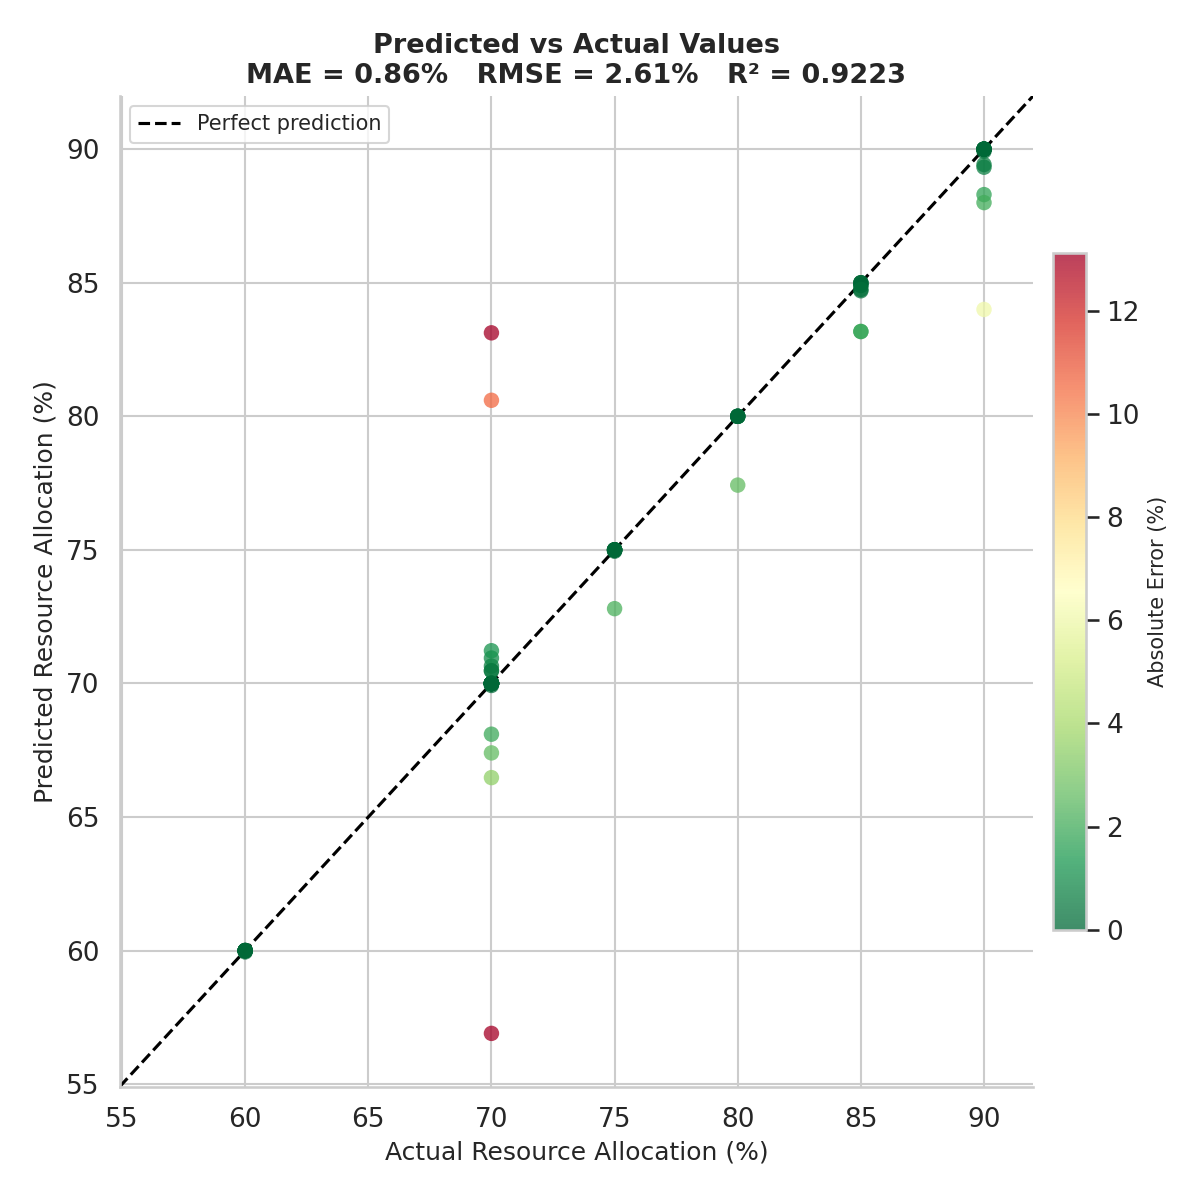
\includegraphics[width=\columnwidth]{fig4.png}
    \caption{\centering Comparison of Predictions and Actual Values}
    \label{figure4}
\end{figure}

This scatter plot compares predicted resource allocation to actual values, with the dashed line representing perfect predictions. Most points cluster near the line, indicating the model generally performs well. However, a few outliers deviate noticeably, suggesting some underestimation or overestimation in those cases. Overall, the distribution indicates a solid predictive capability, though there is room for improvement in handling outliers.

\section{Conclusion}

This study demonstrates that advanced Data Science techniques are essential for optimizing resource allocation in 5G networks — a key aspect of ICT. Using the "5G Resource Allocation Dataset" and Python functions to compute allocation percentages, sort by application type, and train a RandomForestRegressor, our results show that the model effectively prioritizes high-demand, real-time services as signal quality improves.


Overall, our integrated approach of data cleaning, feature engineering, and machine learning provides a scalable framework for dynamic network management, with future work aimed at refining model accuracy and addressing outliers.

\section*{Acknowledgments}

I thank Mykola Melnyk, a third-year ICT student at the Faculty of Electrical Engineering and Information Technology, for his valuable help with the project's practical part and his insightful advice.

\bibliographystyle{plain}
\begin{thebibliography}{9}

\bibitem{SOBHY2023} 
SOBHY, O. (2023). \emph{5G Resource Allocation Dataset: Optimizing Band}. Kaggle. 

Available at: \url{kaggle.com/datasets/omarsobhy14/5g-quality-of-service}.

\bibitem{KaggleLearn}
KAGGLE. (n.d.). \emph{Learn Python, Data Viz, Pandas \& More | Tutorials | Kaggle}. 

Available at: \url{kaggle.com/learn}.

\bibitem{RandomForestRegressor}
\emph{RandomForestRegressor — scikit-learn 1.6.1 documentation}. 

Available at: \url{scikit-learn.org/stable/modules/generated/sklearn.ensemble.RandomForestRegressor.html}.

\end{thebibliography}

\end{document}

 